% --- Latexai AI-change highlighting macro ---
% Set this to \laishowchangesfalse to hide red AI markup.
\newif\iflaishowchanges
\laishowchangestrue
\long\def\lai#1{%
  \iflaishowchanges
    {\color{red}#1}%
  \else
    #1%
  \fi
}
% --- end Latexai AI-change highlighting macro ---

\usepackage{xcolor}
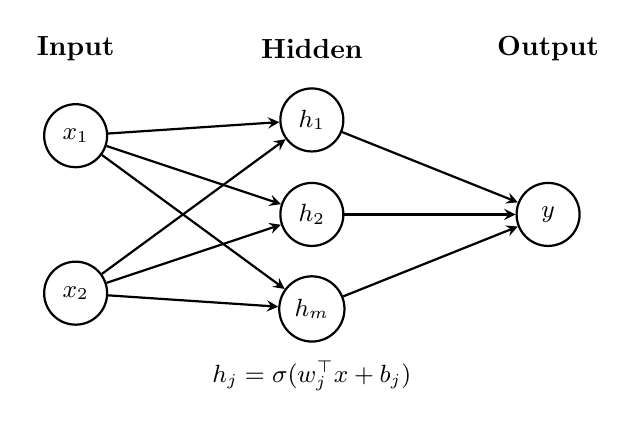
\begin{tikzpicture}[>=stealth, every node/.style={font=\small}]
  \tikzstyle{unit}=[circle, draw, thick, minimum size=8mm, align=center]
  \node[font=\bfseries] at (0, 2.1) {Input};
  \node[font=\bfseries] at (3, 2.1) {Hidden};
  \node[font=\bfseries] at (6, 2.1) {Output};
  \node[unit] (x1) at (0, 1.0) {$x_1$};
  \node[unit] (x2) at (0,-1.0) {$x_2$};
  \node[unit] (h1) at (3, 1.2) {$h_1$};
  \node[unit] (h2) at (3, 0.0) {$h_2$};
  \node[unit] (hm) at (3,-1.2) {$h_m$};
  \node[unit] (y)  at (6, 0.0) {$y$};
  \foreach \i in {x1,x2}{
    \foreach \j in {h1,h2,hm}{
      \draw[->, thick] (\i) -- (\j);
    }
  }
  \foreach \j in {h1,h2,hm}{
    \draw[->, thick] (\j) -- (y);
  }
  \node at (3,-2.05) {$h_j=\sigma(w_j^\top x+b_j)$};
\end{tikzpicture}
